\section{Конструкторская часть}

В этом разделе будут представлены схемы реализуемых алгоритмов.

\subsection{Сортировка выбором}

Схема алгоритма сортировки выбором представлена на рисунке~\ref{fig:choice}.

\begin{figure}
	\centering
	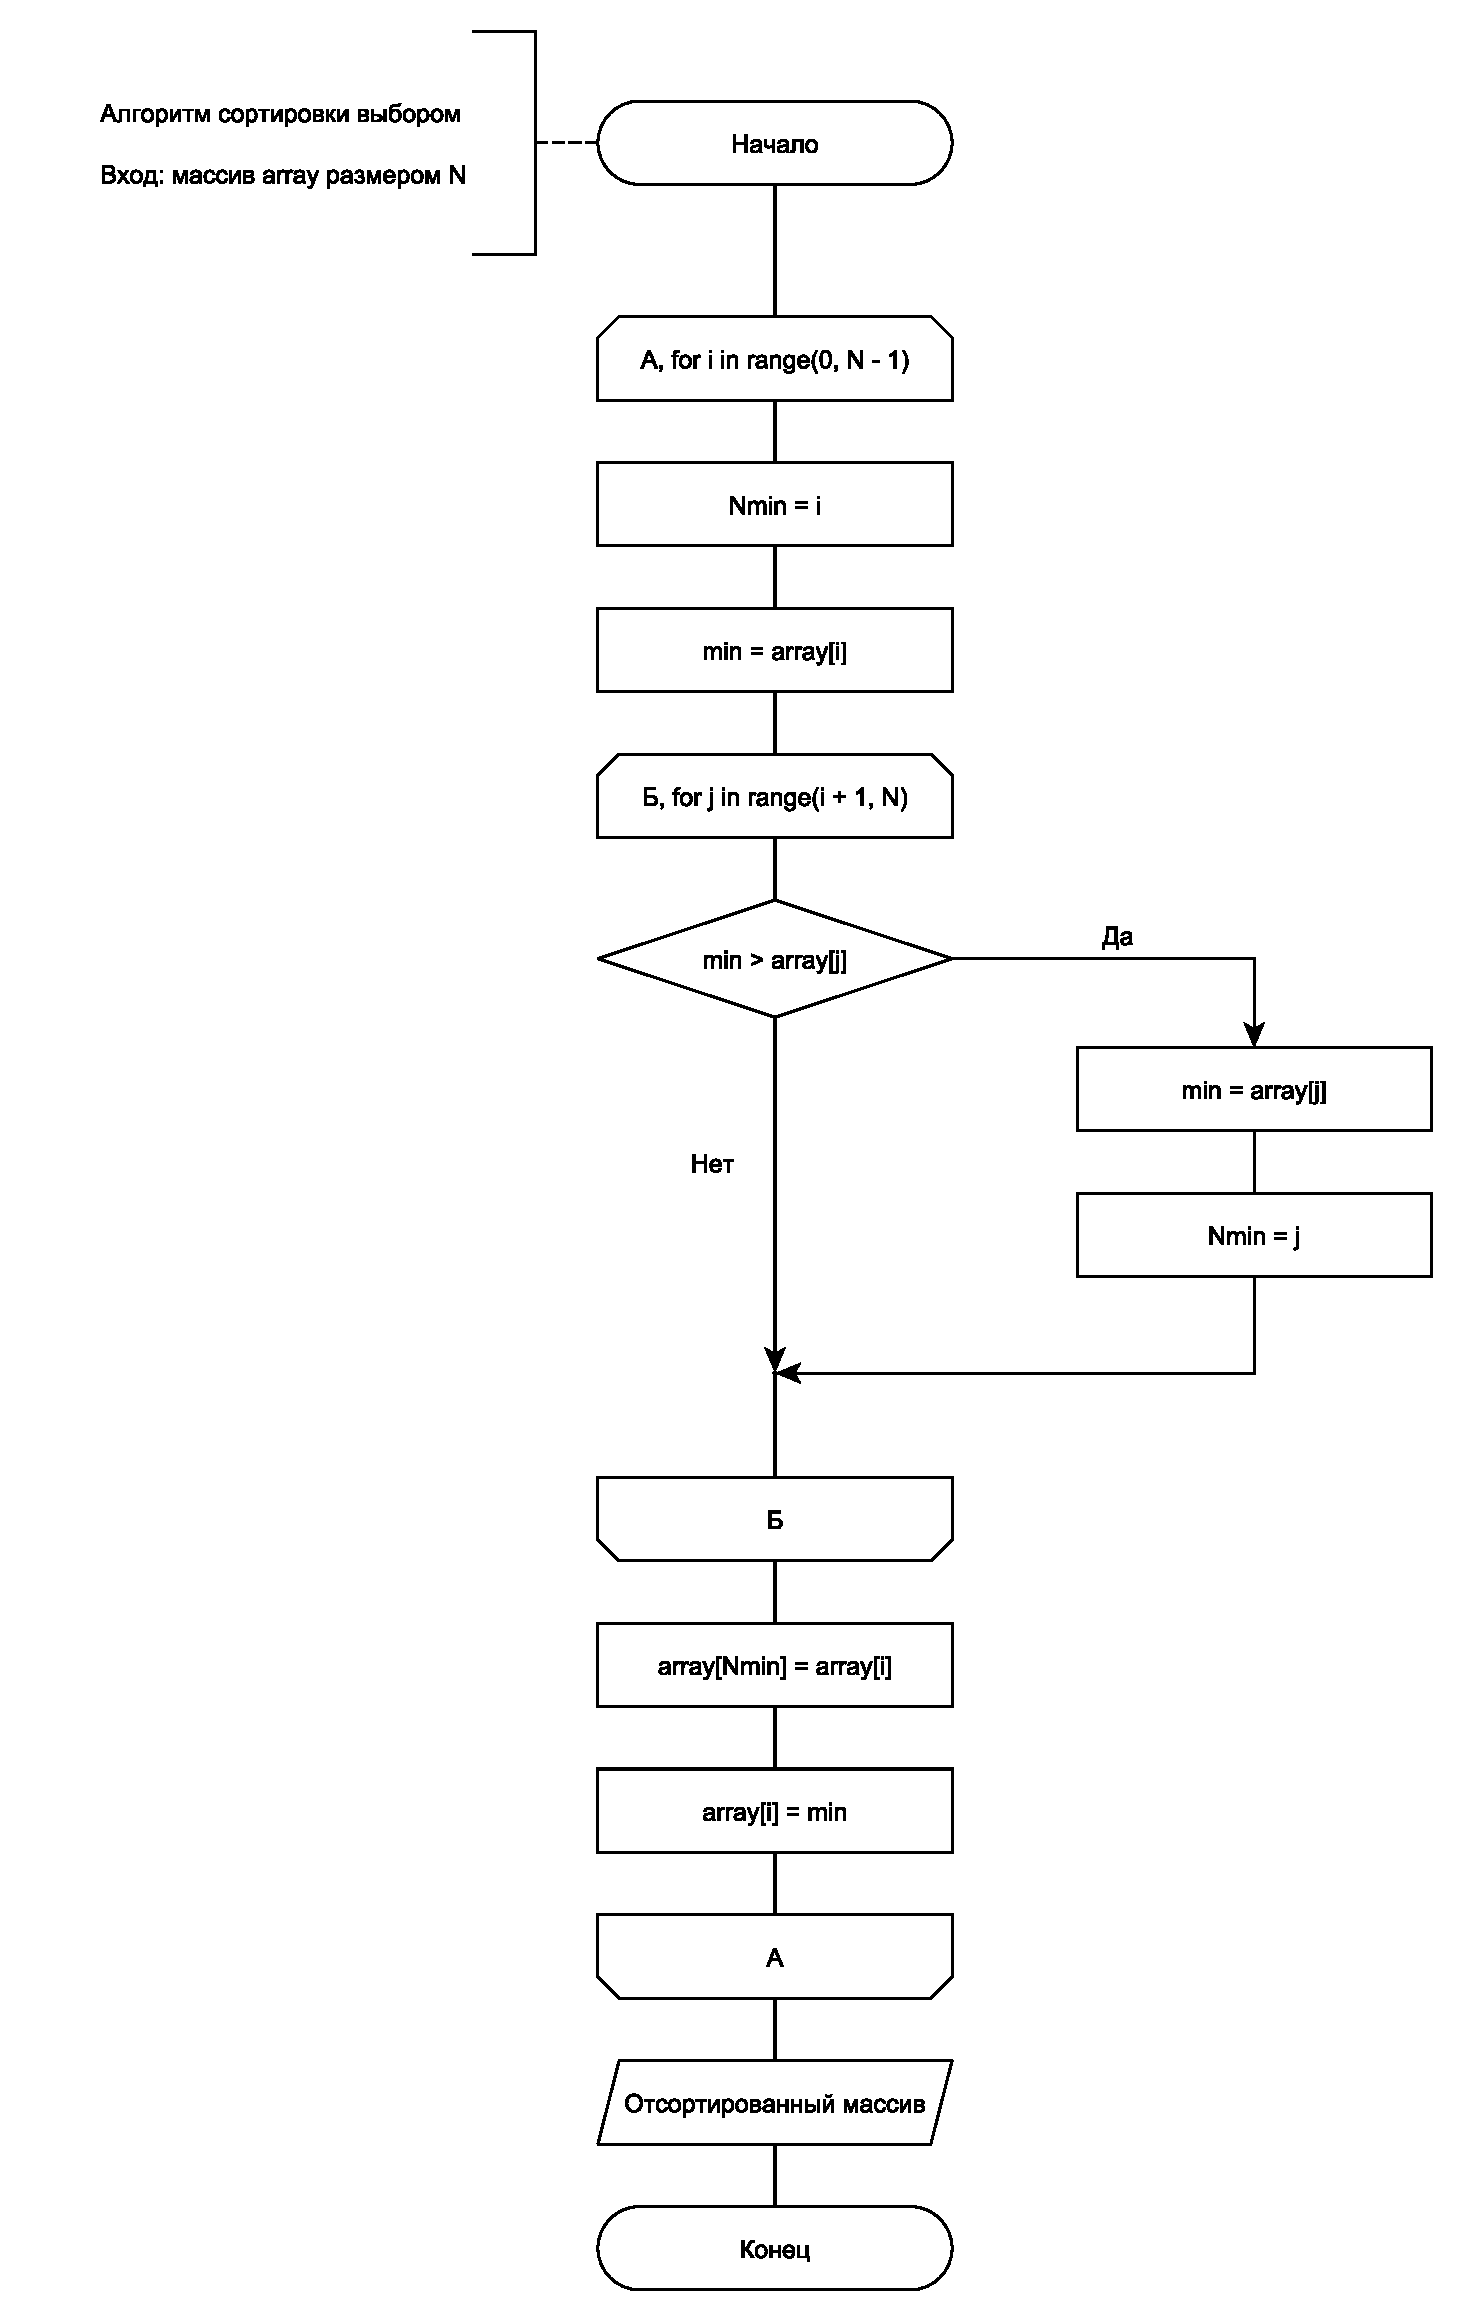
\includegraphics[width=0.7\linewidth]{images/choice}
	\caption{Схема алгоритма сортировки выбором}
	\label{fig:choice}
\end{figure}

\subsection{Сортировка перемешиванием}

Схема алгоритма сортировки перемешиванием представлена на рисунке~\ref{fig:shake}.

\begin{figure}
	\centering
	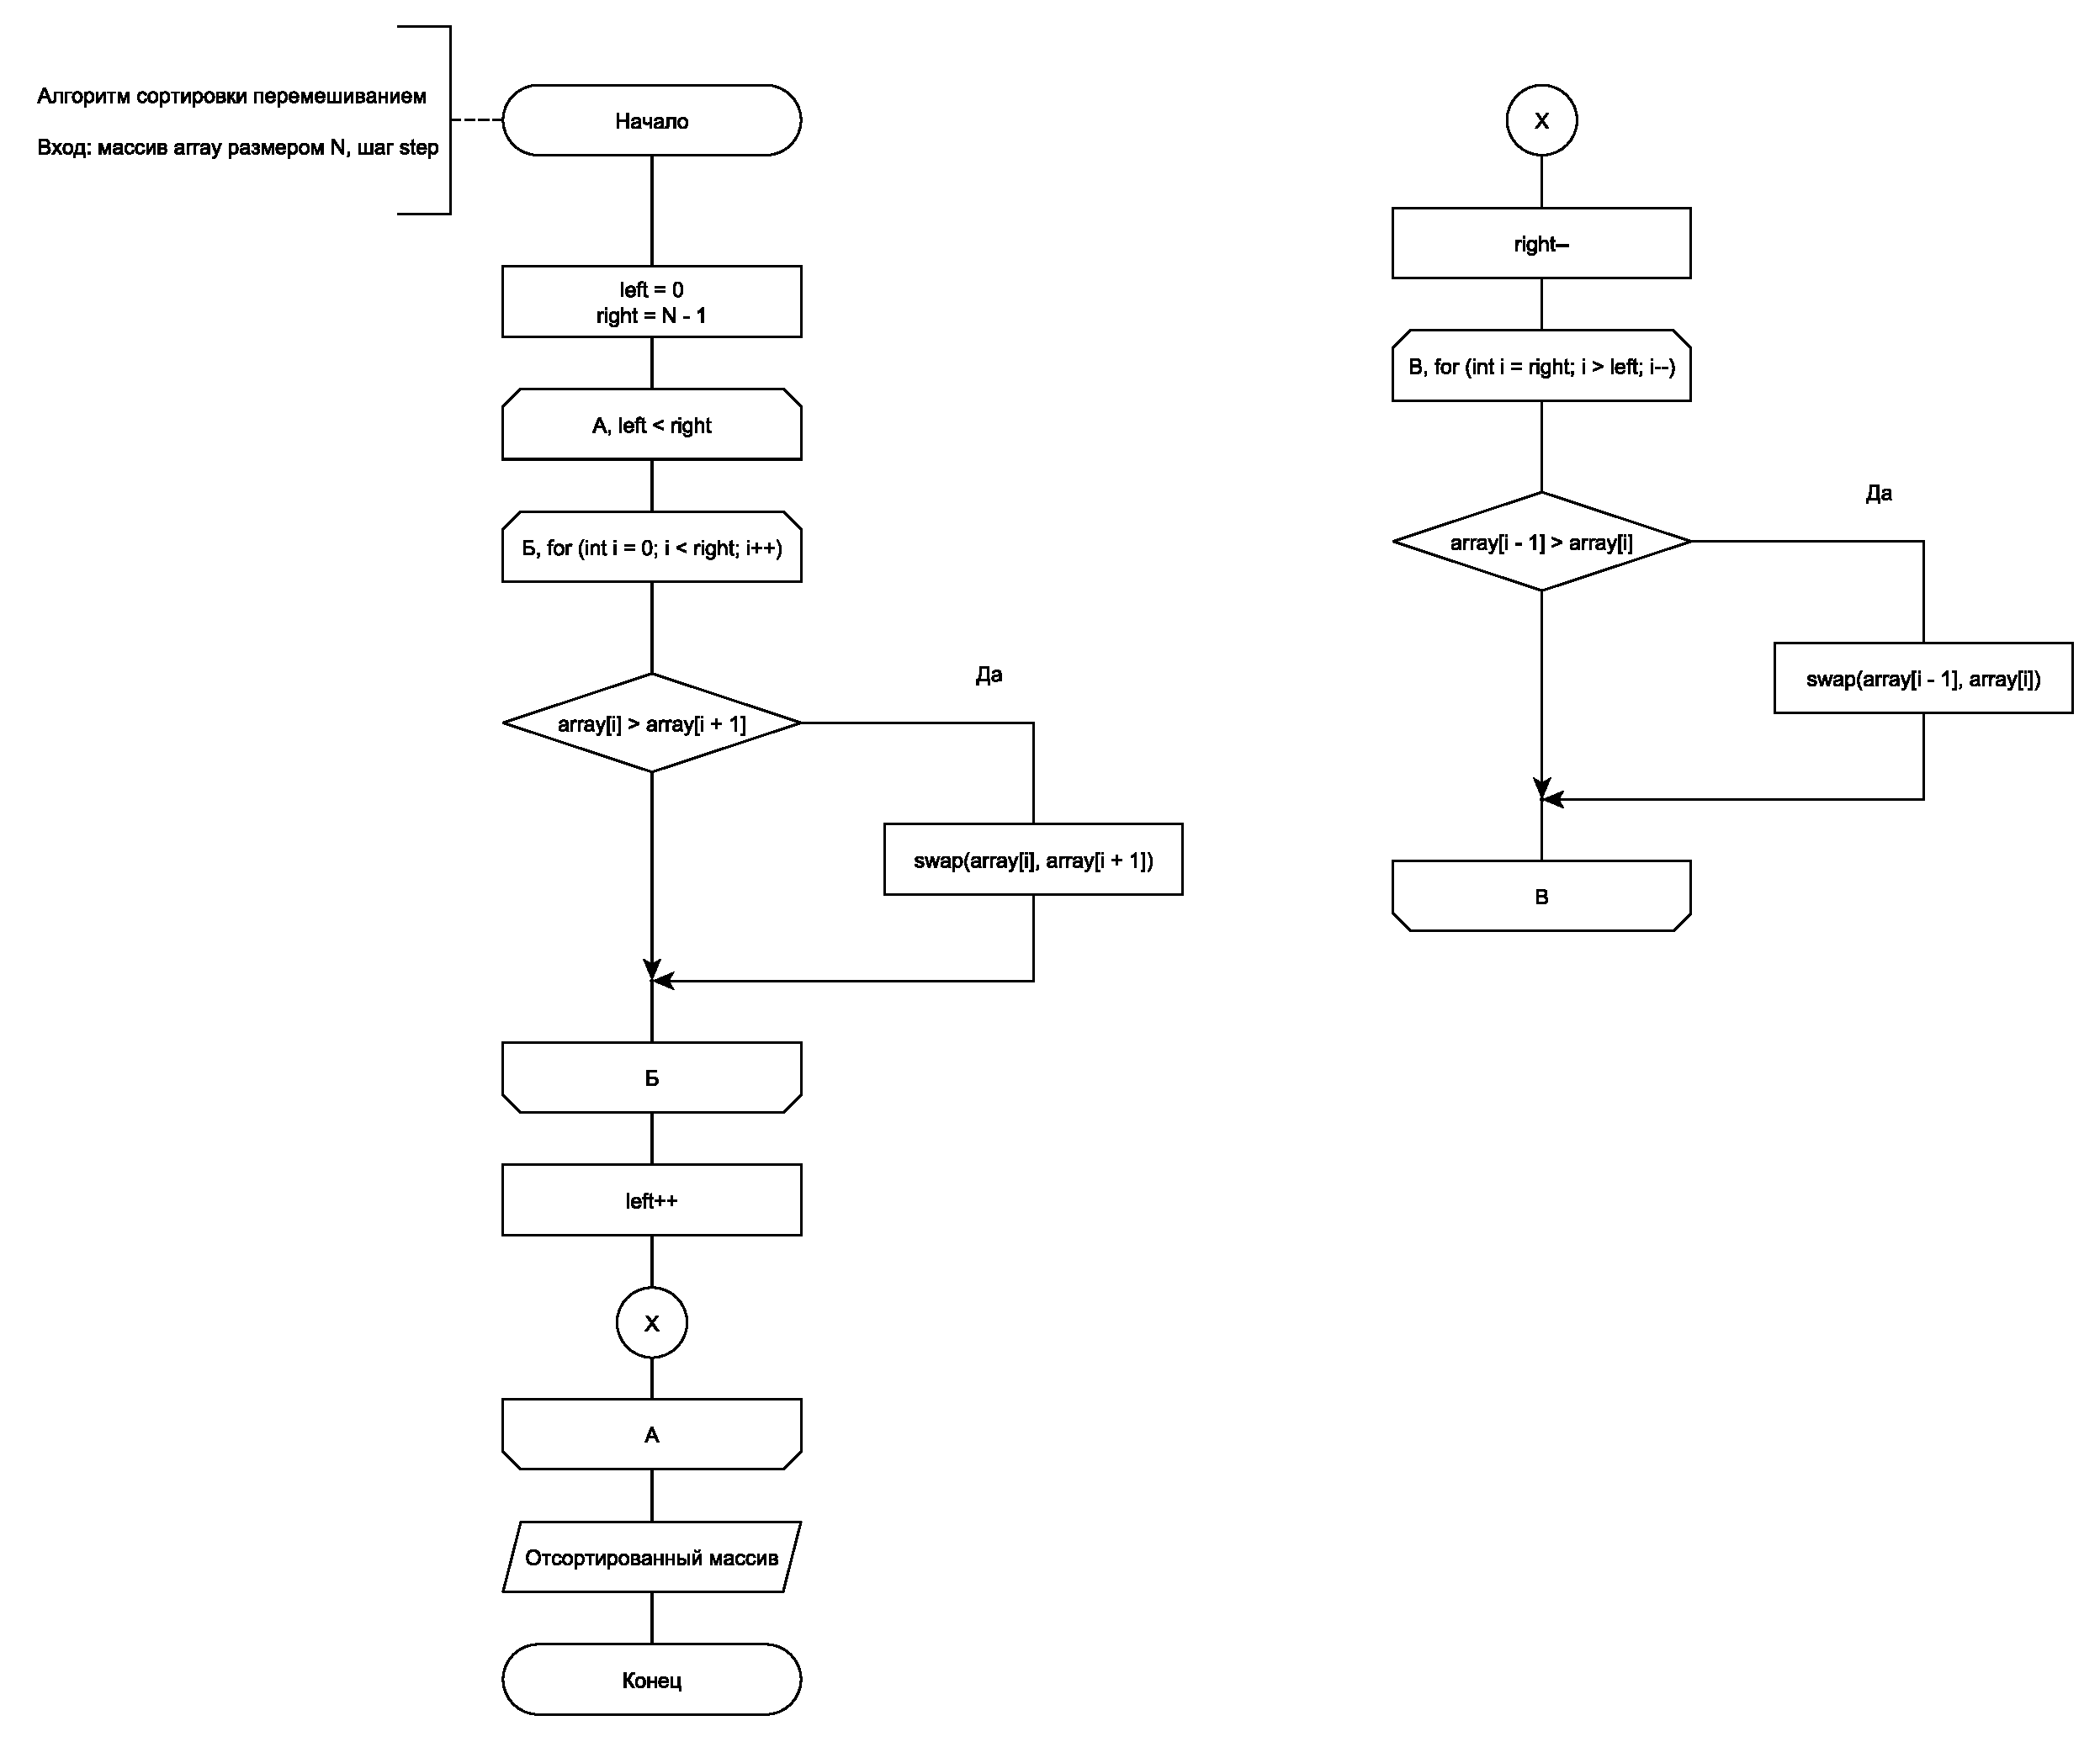
\includegraphics[width=1.0\linewidth]{images/shake}
	\caption{Схема алгоритма сортировки перемешиванием}
	\label{fig:shake}
\end{figure}

\newpage


\subsection{Модель вычислений}
Для последующего вычисления трудоемкости необходимо ввести модель вычислений:
\begin{enumerate}
	\item операции из списка (\ref{for:opers}) имеют трудоемкость 1;
	\begin{equation}
		\label{for:opers}
		+, -, *, /, \%, ==, !=, <, >, <=, >=, [], ++, {-}-
	\end{equation}
	\item трудоемкость оператора выбора \code{if условие then A else B} рассчитывается как (\ref{for:if});
	\begin{equation}
		\label{for:if}
		f_{if} = f_{\text{условия}} +
		\begin{cases}
			f_A, & \text{если условие выполняется,}\\
			f_B, & \text{иначе.}
		\end{cases}
	\end{equation}
	\item трудоемкость цикла рассчитывается как (\ref{for:for});
	\begin{equation}
		\label{for:for}
		f_{for} = f_{\text{инициализации}} + f_{\text{сравнения}} + N(f_{\text{тела}} + f_{\text{инкремента}} + f_{\text{сравнения}})
	\end{equation}
	\item трудоемкость вызова функции равна 0.
\end{enumerate}


\subsection{Трудоемкость алгоритмов}

В следующих частях будут рассчитаны трудоемкости представленных ранее алгоритмов сортировки.

Далее размер массива будет обозначаться символом N.

\subsubsection{Сортировка выбором}

Трудоёмкость сортировки выбором состоит из:

\begin{itemize}
	\item трудоёмкости внешнего цикла по $i \in [0..N-1]$, трудоёмкость которого: $f = 2 + (N - 1) \cdot (2 + f_{inner})$;
	\item трудоёмкости внутреннего цикла по $j \in [i+1..N]$, трудоёмкость которого в среднем: $f_{inner} = 2 + (N - 1) / 2 \cdot (2 + 2 + 2)$;
\end{itemize}

Итого, средняя трудоёмкость сортировки выбором: 
\begin{equation}
	% f = 2 + (N - 1) \cdot (2 + 2 + (N - 1) / 2 \cdot (2 + (2 + 7)) = 2 + (N - 1) \cdot (4 + (N - 1) \cdot 3) = 2 + (N - 1) \cdot (3 + 3N) = 3N^2 - 1
	f = 3N^2 - 1
\end{equation}

\subsubsection{Сортировка перемешиванием}

Трудоёмкость сортировки перемешивания состоит из:

\begin{itemize}
	\item трудоёмкости внешнего цикла $A$, трудоёмкость которого: $f = 2 + (N - 1) \cdot (2 + f_{inner})$;
	\item трудоёмкости двух внутренних циклов по $i \in [0..N]$, трудоёмкость которых в среднем: $f_{inner} = 2 + (N - 1) \cdot (2 + 2 + f_{swap})$;
	\item трудоёмкости функции обмена $f_{swap} = 7$.
\end{itemize}

Итого, средняя трудоёмкость сортировки перемешиванием: 
\begin{equation}
	% f = 2 + (N - 1) \cdot (2 + (N - 1) \cdot 11)
	f = 11N^2 - 20N + 11
\end{equation}

Решение уравнения $11N^2 - 20N + 11 = 3N^2 - 1$ даёт ответ $N = 1.5$.
Т.е. трудоёмкость сортировки перемешиванием больше трудоёмкости сортировки выбором после размера массива больше единицы.
